\subsection{\textit{Bidirectional Encoder Representations from Transformers} \\ (BERT)}

BERT, yang merupakan singkatan dari \textit{Bidirectional Encoder Representations from Transformers}, adalah model pemrosesan bahasa alami yang diperkenalkan oleh Google pada tahun 2018 \parencite{bert}. BERT memanfaatkan arsitektur \textit{transformer}, yang telah dibahas sebelumnya, untuk memahami konteks kata dalam teks dengan cara yang lebih mendalam daripada pendekatan sebelumnya.

BERT menggunakan pendekatan yang \textit{bidirectional}. BERT mampu memahami teks dari kiri ke kanan atau sebaliknya, BERT memahami konteks kata dengan mempertimbangkan informasi dari kedua arah. Sehingga, model ini memiliki kemampuan untuk pemahaman yang lebih kaya tentang makna dan nuansa dalam teks.

\begin{figure}[ht]
    \centering
    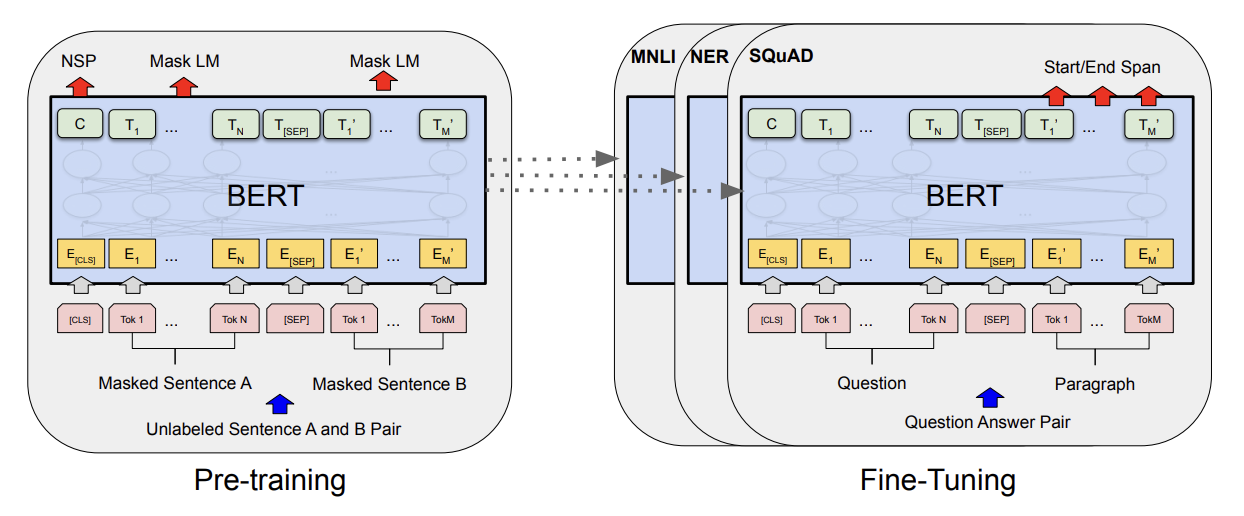
\includegraphics[width=0.8\textwidth]{chapter-2/bert.png}
    \caption{Arsitektur \textit{BERT} \parencite{bert}}
    \label{fig:bert}
\end{figure}

BERT merupakan \textit{pre-trained model} sehingga telah dilatih pada sejumlah besar teks. Data latih BERT diambil dari BooksCorpus dan Wikipedia bahasa Inggris. Ini memungkinan BERT untuk mempunyai pengetahuan mendasar dalam tugas NLP. Ketika digunakan untuk tugas-tugas NLP spesifik, seperti klasifikasi teks atau pemahaman pertanyaan, BERT dapat disesuaikan dengan data tugas spesifik untuk meningkatkan kinerjanya.

Model ini dikembangkan dengan dua konfigurasi, yaitu BASE dan LARGE. BERT dengan konfigurasi BASE memiliki 12 \textit{layer encoder} yang mempunyai 768 \textit{hidden layer} pada FFNN dan 12 \textit{attention heads}. Sedangkan, untuk konfigurasi BERT LARGE memiliki 24 \textit{layer encoder} yang mempunyai 1024 \textit{hidden layer} pada FFNN dan 16 \textit{attention heads}.